\documentclass[12pt]{report}
\usepackage[utf8]{inputenc}
\usepackage[russian]{babel}
%\usepackage[14pt]{extsizes}
\usepackage{listings}
\usepackage{graphicx}
\usepackage{amsmath,amsfonts,amssymb,amsthm,mathtools} 
\usepackage{pgfplots}
\usepackage{filecontents}
\usepackage{indentfirst}
\usepackage{eucal}
\usepackage{amsmath}
\usepackage{enumitem}
\frenchspacing

\usepackage{indentfirst} % Красная строка


%\usetikzlibrary{datavisualization}
%\usetikzlibrary{datavisualization.formats.functions}

\usepackage{amsmath}




% Для листинга кода:
\lstset{ %
language=haskell,                 % выбор языка для подсветки (здесь это С)
basicstyle=\small\sffamily, % размер и начертание шрифта для подсветки кода
numbers=left,               % где поставить нумерацию строк (слева\справа)
numberstyle=\tiny,           % размер шрифта для номеров строк
stepnumber=1,                   % размер шага между двумя номерами строк
numbersep=5pt,                % как далеко отстоят номера строк от подсвечиваемого кода
showspaces=false,            % показывать или нет пробелы специальными отступами
showstringspaces=false,      % показывать или нет пробелы в строках
showtabs=false,             % показывать или нет табуляцию в строках
frame=single,              % рисовать рамку вокруг кода
tabsize=2,                 % размер табуляции по умолчанию равен 2 пробелам
captionpos=t,              % позиция заголовка вверху [t] или внизу [b] 
breaklines=true,           % автоматически переносить строки (да\нет)
breakatwhitespace=false, % переносить строки только если есть пробел
escapeinside={\#*}{*)}   % если нужно добавить комментарии в коде
}

\usepackage[left=2cm,right=2cm, top=2cm,bottom=2cm,bindingoffset=0cm]{geometry}
% Для измененных титулов глав:
\usepackage{titlesec, blindtext, color} % подключаем нужные пакеты
\definecolor{gray75}{gray}{0.75} % определяем цвет
\newcommand{\hsp}{\hspace{20pt}} % длина линии в 20pt
% titleformat определяет стиль
\titleformat{\chapter}[hang]{\Huge\bfseries}{\thechapter\hsp\textcolor{gray75}{|}\hsp}{0pt}{\Huge\bfseries}


% plot
\usepackage{pgfplots}
\usepackage{filecontents}
\usetikzlibrary{datavisualization}
\usetikzlibrary{datavisualization.formats.functions}
\RequirePackage[
  style=gost-numeric,
  language=auto,
  autolang=other,
  sorting=none,
]{biblatex}

\addbibresource{bib.bib}
\begin{document}
%\def\chaptername{} % убирает "Глава"
\thispagestyle{empty}
\begin{titlepage}
	\noindent \begin{minipage}{0.15\textwidth}
	
\includegraphics[width=\linewidth]{b_logo}
	\end{minipage}
	\noindent\begin{minipage}{0.9\textwidth}\centering
		\textbf{Министерство науки и высшего образования Российской Федерации}\\
		\textbf{Федеральное государственное бюджетное образовательное учреждение высшего образования}\\
		\textbf{~~~«Московский государственный технический университет имени Н.Э.~Баумана}\\
		\textbf{(национальный исследовательский университет)»}\\
		\textbf{(МГТУ им. Н.Э.~Баумана)}
	\end{minipage}
	
	\noindent\rule{18cm}{3pt}
	\newline\newline
	\noindent ФАКУЛЬТЕТ $\underline{\text{«Информатика и системы управления»}}$ \newline\newline
	\noindent КАФЕДРА $\underline{\text{«Программное обеспечение ЭВМ и информационные технологии»}}$\newline\newline\newline\newline\newline
	
	
	\begin{center}
		\noindent\begin{minipage}{1.3\textwidth}\centering
			\Large\textbf{  Отчёт по лабораторной работе №1 по дисциплине}\newline
			\textbf{ "Проектирование рекомендательных систем"}\newline\newline
		\end{minipage}
	\end{center}
	
	\noindent\textbf{Тема} $\underline{\text{Сравнение алгоритмов поиска ассоциативных правил}}$\newline\newline
	\noindent\textbf{Студент} $\underline{\text{Варламова Е. А.}}$\newline\newline
	\noindent\textbf{Группа} $\underline{\text{ИУ7-33М}}$\newline\newline
	\noindent\textbf{Оценка (баллы)} $\underline{\text{~~~~~~~~~~~~~~~~~~~~~~~~~~~}}$\newline\newline
	\noindent\textbf{Преподаватели} $\underline{\text{Быстрицкая А.Ю.}}$\newline\newline\newline
	
	\begin{center}
		\vfill
		Москва~---~\the\year
		~г.
	\end{center}
\end{titlepage}
\large
\setcounter{page}{2}
\def\contentsname{СОДЕРЖАНИЕ}
\renewcommand{\contentsname}{СОДЕРЖАНИЕ}
\tableofcontents
\renewcommand\labelitemi{---}
\newpage
\chapter*{Введение}
\addcontentsline{toc}{chapter}{ВВЕДЕНИЕ}



Цель работы -- сравнение алгоритмов поиска ассоциативных правил Apriori, ECLAT и FP-Growth.

Для достижения поставленной цели потребуется:
\begin{itemize}
	\item привести описание алгоритмов Apriori, ECLAT и FP-Growth;
	\item привести описание используемых для исследования данных;
	\item провести сравнение алгоритмов по времени работы и затратам по памяти.
\end{itemize}

\pagebreak

\chapter{Аналитический раздел}

\section{Задача поиска ассоциативных правил}

Правило ассоциации состоит из двух частей, предшествующей и последующей. Предшествующая задача -- это элемент, находящийся в данных. А последующая -- это элемент или множество элементов, которые встречаются в сочетании с предшествующей задачей. \cite{sr1}

В интеллектуальном анализе данных правила ассоциации являются полезными и помогают спрогнозировать поведение клиента.

Для оценки качества полученных рекомендаций используются следующие метрики \cite{sr1}:

\begin{itemize}
	\item Поддержка -- позволяет узнать, насколько часто объект встречается в БД. Определяется как количество транзакций, содержащих X к общему числу транзакций: $support(X) = \frac{|t \in T, x \in X |}{|T|}$
	\item Достоверность -- показывает, насколько хорошим является правило для предсказания правой части,когда условие слева верно. Определяется как $confidence(A \rightarrow B) = \frac{supp(A \cup B)}{supp(A)}$
	\item Интерес -- измеряет силу правила, сравнивая полное правило с предположенной правой частью и рассчитывается, как отношение достоверности правила к частоте появления следствия -- $lift(A \rightarrow B) = \frac{supp(A \cup B)}{supp(A)supp(B)}$
    \item Уверенность -- частотность ошибок правила: $conv(A \rightarrow B) = \frac{1 - supp(B)}{1 -conf(A \rightarrow B)}$
\end{itemize}

\section{Apriori}
Принцип работы алгоритма \cite{apyori}:
\begin{enumerate}
    \item Определение минимальной поддержки: устанавливается порог минимальной поддержки, который определяет, как часто элемент или набор элементов должен встречаться в транзакциях для того, чтобы считаться значимым.

    \item Сбор данных: собираются данные о транзакциях. Транзакции могут представлять собой покупки товаров в магазине, клики на веб-сайте и т.д. Каждая транзакция состоит из множества элементов (например, товаров).

    \item Генерация частых одиночных элементов: алгоритм начинает с поиска всех одиночных элементов (товаров), которые удовлетворяют минимальной поддержке. Это создаёт первый набор частых элементов.

    \item Генерация кандидатов: на основе найденных частых одиночных элементов создаются кандидаты для пар (двухэлементных наборов), троек и так далее. Этот процесс повторяется, увеличивая размер набора элементов.

    \item Отбрасывание нечастых кандидатов: для каждого нового набора кандидатов вычисляется их поддержка. Если поддержка не достигает установленного порога, набор отбрасывается.

    \item Повторение процесса: процесс генерации кандидатов и вычисления их поддержки повторяется до тех пор, пока не останется ни одного кандидата, который бы удовлетворял минимальной поддержке.

    \item Генерация ассоциативных правил: на основе частых наборов элементов создаются ассоциативные правила. Каждое правило имеет форму "если A, то B", где A и B — это наборы элементов. Для каждого правила вычисляется мера уверенности (confidence), которая показывает вероятность того, что если A присутствует в транзакции, то также присутствует и B.

    \item Фильтрация правил: наконец, правила могут быть отфильтрованы по уверенности или другим критериям, чтобы оставить только наиболее значимые.
\end{enumerate}

\section{ECLAT}

Принцип работы алгоритма \cite{pyECLAT}:

\begin{enumerate}
    \item Построение таблицы транзакций: каждому элементу в наборе данных присваивается уникальный идентификатор, и создается таблица, где каждая строка представляет собой список идентификаторов транзакций, содержащих этот элемент.

    \item Определение минимальной поддержки: устанавливается порог минимальной поддержки, аналогично алгоритму Apriori.

    \item Генерация частых наборов: для каждого элемента в таблице вычисляется поддержка. Затем алгоритм начинает генерировать частые наборы, используя пересечение списков транзакций:
    \begin{itemize}
        \item Если есть два элемента A и B, необходимо брать их списки транзакций и находить пересечение (т.е., транзакции, которые содержат оба элемента).
        \item Если пересечение превышает порог минимальной поддержки, создается новый набор A, B.
    \end{itemize}
    \item Повторение процесса: процесс повторяется для всех возможных комбинаций элементов до тех пор, пока не будут найдены все частые наборы.
    \item Генерация ассоциативных правил: на основе найденных частых наборов создаются ассоциативные правила, аналогично тому, как это делается в Apriori.
\end{enumerate}

\section{FP-Growth}

Принцип работы алгоритма \cite{fpgrowth}:
\begin{enumerate}
    \item Сбор данных и определение минимальной поддержки: определите набор транзакций и установите порог минимальной поддержки.

    \item Подсчет частоты элементов: подсчитайте, как часто каждый элемент встречается в транзакциях.

    \item Построение FP-дерева: создайте FP-дерево, начиная с корня, где каждый узел представляет элемент и его частоту. Элементы добавляются в дерево по порядку их частоты (от наиболее частых к наименее частым).

    \item Извлечение частых наборов: для каждого элемента (листового узла) в FP-дереве создается условное FP-дерево, включающее только транзакции, содержащие данный элемент. Этот процесс повторяется рекурсивно для каждого элемента до тех пор, пока не будут найдены все частые наборы.

    \item Генерация ассоциативных правил: на основе найденных частых наборов создаются ассоциативные правила.
\end{enumerate}
\pagebreak

\chapter{Конструкторский раздел}

В данном разделе описаны данные, анализируемые в данной работе.

\section{Market Basket Optimisation}

В качестве источника данных был взят датасет, располагающийся в свободном доступе на веб-сайте Kaggle \cite{dataset}. Набор данных включает в себя корзины потребителя некоторого продуктового магазина. В качестве предобработки была построена база данных транзакций, которая структурно изменялась по требованию входных данных используемых алгоритмов.

\pagebreak

\chapter{Технологический раздел}

В данном разделе описываются средства разработки программного обеспечения.

\section{Средства реализации}

В качестве используемого был выбран язык программирования Python \cite{Python}.

Данный выбор обусловлен следующими факторами:
\begin{itemize}
	\item Большое количество исчерпывающей документации;
	\item Широкий выбор доступных библиотек для разработки;
	\item Простота синтаксиса языка и высокая скорость разработки.
\end{itemize} 

При написании программного продукта использовалась среда разработки Visual Studio Code. Данный выбор обусловлен тем, что данная среда распространяется по свободной лицензии, поставляется для конечного пользователя с открытым исходным кодом, а также имеет большое число расширений, ускоряющих разработку.

\section{Библиотеки}

При анализе и обработке датасета, а также для решения поставленных задач использовались библиотеки:
\begin{itemize}
	\item pandas;
	\item numpy;
	\item matplotlib;
	\item apyory \cite{apyori};
	\item pyECLAT \cite{pyECLAT};
	\item fpgrowth-py \cite{fpgrowth_py}.
\end{itemize}


\chapter{Исследовательский раздел}
\section{Условия исследований}
Исследование проводилось на персональном вычислительной машине со следующими характеристиками:

\begin{itemize}
\item процессор Intel Core i5
\item операционная система Mac OS Big Sur,
\item 8 Гб оперативной памяти.
\end{itemize}

Временные затраты определялись с использованием библиотеки time. Затраты по памяти определялись с использованием библиотеки memory\_profiler.

В данном исследовании значение параметра минимальной поддержки изменялось от значения $0.001$ до $0.01$ с шагом $0.001$ и от $0.01$ до $0.25$ с шагом $0.01$. Значение минимального и максимального количества элементов было равно $2$ для ECLAT, для остальных не ограничено сверху.

\section{Зависимость времени исполнения от параметра минимальной поддержки}

На рисунке \ref{img:time} представлен график зависимости времени исполнения алгоритмов от заданного параметра минимальной поддержки.

\begin{figure}[H]
	\centering
	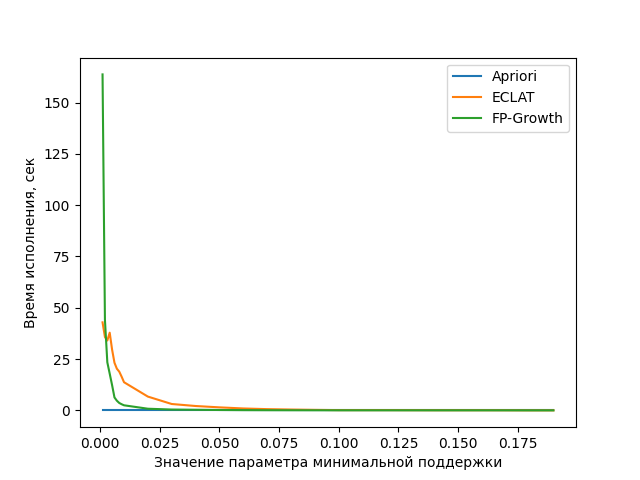
\includegraphics[width=\textwidth]{time.png}
	\caption{ График зависимости времени исполнения от заданного параметра минимальной поддержки.}
	\label{img:time}
\end{figure}


\section{Зависимость количества занятой памяти процессом во время исполнения алгоритмов от заданного параметра минимальной поддержки}

На рисунке \ref{img:memory} представлен график зависимости количества занятой памяти процессом во время исполнения алгоритмов от заданного параметра минимальной поддержки.


\begin{figure}[H]
	\centering
	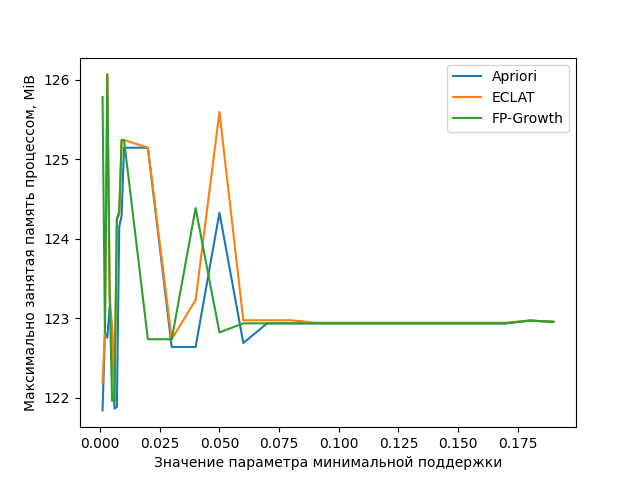
\includegraphics[width=\textwidth]{mem.png}
	\caption{ График зависимости количества занятой процессом во время исполнения алгоритмов от заданного параметра минимальной поддержки.}
	\label{img:memory}
\end{figure}

\subsection*{Вывод}

В результате проведенных исследований заметно, что по времени исполнения на меньших значениях параметра минимальной поддержки самое долгое время исполнения у алгоритма FP-Growth. Самым быстрым временем исполнения обладает алгоритм Apriori. В дальнейшем, при увеличении параметра, разница во времени исполнения у трех алгоритмов становится уже не такой заметной и при значении параметра минимальной поддержки равным $0.10$ уже практически отсутствует.

Также стоит отметить, что размер задействованной памяти, потребовавшейся для исполнения каждого из алгоритмов, практически одинаков. Отличия присутствуют лишь при начальных значениях величины параметра минимальной поддержки.



\chapter*{ЗАКЛЮЧЕНИЕ}
\addcontentsline{toc}{chapter}{ЗАКЛЮЧЕНИЕ}
В ходе выполнения работы было проведено сравнение алгоритмов поиска ассоциативных правил Apriori, ECLAT и FP-Growth.

Исследования показали, что при заданных условиях отличия во времени исполнения между алгоритмами не разительны, однако на меньших значениях параметра минимальной поддержки наилучшим образом себя показал именно алгоритм Apriori.

Были решены следующие задачи:
\begin{itemize}
	\item приведено описание алгоритмов Apriori, ECLAT и FP-Growth;
	\item приведено описание используемых для исследования данных;
	\item проведено сравнение алгоритмов по времени работы и затратам по памяти.
\end{itemize}

\pagebreak

\printbibliography[title={СПИСОК ИСПОЛЬЗОВАННЫХ\\ ИСТОЧНИКОВ}]
\addcontentsline{toc}{chapter}{СПИСОК ИСПОЛЬЗОВАННЫХ ИСТОЧНИКОВ}

\bibliographystyle{utf8gost705u}  % стилевой файл для оформления по ГОСТу       % имя библиографической базы (bib-файла) 

\pagebreak
\end{document}